\documentclass[]{article}
%use European style
%\usepackage[a4paper,left=2cm,right=2cm,top=2cm,bottom=2cm]{geometry}

%few useful packages ------------------------------------------------------------------
\usepackage{setspace}
\let\Tiny=\tiny %remove annoying warnings
\usepackage[english]{babel}
\usepackage[latin1]{inputenc}
\usepackage{amsmath}
\usepackage{amssymb}
\usepackage{amsthm}
\usepackage{amsfonts}
\usepackage{colortbl}
\usepackage{xcolor}
\usepackage{eurosym}
\usepackage{enumitem}
\usepackage{chngpage}
\usepackage{fancyhdr}
\usepackage{fancyvrb}
\usepackage{float}
\usepackage{framed}
\usepackage{multirow}
\usepackage{graphicx}
\graphicspath{ {./images/} }
\usepackage{geometry}
\usepackage{lipsum}
\usepackage{tabularx}
\usepackage[linktocpage]{hyperref}

%define environment for code
\definecolor{orangepse}{RGB}{240,139,39}
\definecolor{redpse}{RGB}{222,6,61}
\newcommand{\rpse}[1]{\textcolor{redpse}{#1}}
\definecolor{dkgreen}{rgb}{0,0.6,0}
\definecolor{gray}{rgb}{0.5,0.5,0.5}
\definecolor{mauve}{rgb}{0.58,0,0.82}

\usepackage{listings}
\lstset{frame=tblr,
	language=R,
	aboveskip=5mm,
	belowskip=5mm,
	showstringspaces=false,
	columns=flexible,
	basicstyle={\small\ttfamily},
	numbers=none,
	numberstyle=\tiny\color{gray},
	keywordstyle=\color{blue},
	commentstyle=\color{dkgreen},
	stringstyle=\color{mauve},
	breaklines=true,
	breakatwhitespace=true,
	tabsize=3
}
%---------------------------------------------------------------------------------------
\usepackage[backend=biber, style=authoryear, maxcitenames=3, citestyle=apa]{biblatex}

\addbibresource{bib.bib} 

% New Commands ----------------------------
\newcommand{\bb}{\bigbreak\noindent}

\makeatletter
\renewcommand\section{\leftskip 0pt\@startsection {section}{1}{\z@}%
	{-3.5ex \@plus -1ex \@minus -.2ex}%
	{2.3ex \@plus.2ex}%
	{\normalfont\Large\bfseries}}

\renewcommand\subsection{\leftskip 4ex\@startsection{subsection}{2}{\z@}%
	{-3.25ex\@plus -1ex \@minus -.2ex}%
	{1.5ex \@plus .2ex}%
	{\normalfont\large\bfseries}}

\renewcommand\subsubsection{\leftskip 14ex\@startsection{subsubsection}{3}{\z@}%
	{-3.25ex\@plus -1ex \@minus -.2ex}%
	{1.5ex \@plus .2ex}%
	{\normalfont\large\bfseries}}
\makeatother


%opening
\title{Referee Report on:\\
	 \textit{``Asset Demand of U.S. Households''}\\
	 \bb
	  \large{by Xavier Gabaix, Ralph S. J. Koijen, Federico Mainardi, Sangmin Oh, and Motohiro Yogo}}
\author{Davide Davies-Biletta}

\begin{document}
\vspace{50ex}

\maketitle
\thispagestyle{empty}
\pagebreak
\pagenumbering{arabic}
\begin{spacing}{1.25}
\section{Recommendation}
I recommend that the authors revise and resubmit their paper.

\section{Summary}
In their recent paper, \cite{gabaix2024asset} aim to contribute the growing literature regarding the role of demand on asset pricing. In particular aim to address a claim made in one of their previous papers: ``It is clear that it would be desirable to know more about the determinants of flows at a high frequency.'' \parencite{gabaix2021search}.  Much of the current work regarding asset pricing evolves around models of the stochastic discount factor as seen in class. However, current models are still incapable of providing answers to some key questions. For example, what role do retail investors play in recent stock rallies and to what extent? By including preference heterogeneity, and accounting for the impact investors may themselves have on prices, demand approaches to asset pricing hope to more accurately answer broad sets of questions which were previously difficult to answer with more traditional reduced-form regressions or event studies \parencite{koijen2019demand}. In this paper \cite{gabaix2024asset} make use of a new and evolving source of high frequency asset portfolio data. This data consists of detailed breakdowns of individual investment portfolios including granular information on assets owned, and the flow of these assets on a day-to-day basis. Furthermore, this novel dataset includes a large sample of ultra-high-net-worth (UHNW) individuals, with around a thousand portfolios with assets in excess of \$100 million and 439 unique portfolios with assets exceeding \$1 billion at some point in their sample. This level of granularity and frequency, coupled with the representation of individuals at the far right tail of the income curve, clearly separates this research from the previous literature.  
 Their findings point to pronounced heterogeneity in asset purchasing behaviours between more-wealthy and less wealthy investors. These differences are accentuated for those more actively investing in equity markets. The evidence from this paper imply the existence of largely inert households, which have relatively little reaction to aggregate shocks. These results are consistent with the idea of investor inertia and inattention, and should provide important suggestions to future macro-financial modelling. 


\section{Major Comments}


\subsection{Under-representation of lower income households}
The authors are keen to explain to the reader how well their novel dataset accounts for individuals associated with the extreme right of the wealth distribution. Yet, they downplay their inability to speak about those on the lower end. 
In section 2.4, the authors outline a series of sample selection screens they use in constructing their final sample. The fifth of such screens removes portfolios with fewer than \$100k in assets (across liquid and illiquid asset classes as well as cash). They justify the use of this screen suggesting it mitigates the concern of capturing only part of a household's assets. Yet, despite this valid concern, this screen effectively removes a considerable portion of the initial observations. Figure 3 implies a loss of approximately 50,000 observations or 25 percent of the eligible sample. It seems highly likely that at least a considerable portion of these observations might contain a household's  unique portfolio. 
\bb
 The authors must therefore ask themselves have they simply substituted under-representation of one extreme for the other? I recommend the authors to include an acknowledgment of this position or further clarify the theoretical justification for this screening process and elimination of lower-wealth households. 
	
	
	\subsection{Limitations to Principle Component Analysis}
	In the final section the authors use a Principal Component Analysis (PCA) to uncover how investors rebalance their portfolios across asset classes. The biggest advantage of PCA is that it reduces the dimensionality of a dataset by extracting orthogonal components \parencite{tsoulfidis2022new}. Yet, it's use to measure portfolio rebalancing flows may oversimplify the underlying dynamics of investor behaviour, potentially overlooking more nuanced relationships and interactions between asset classes. Simply reducing the relationships in your sample to 3 components provides a good basis for further research but seems insufficient for a published paper of this quality. For example, in their seminal paper \cite{stock2002forecasting} describe how they use PCA only as an initial step to then forecast future macroeconomic trends. For this reason, I suggest that authors seek to support their findings using alternative methodologies or build upon their the results of their principle component analysis with the aim of providing a more comprehensive understanding of portfolio rebalancing dynamics.
	
	
	\subsection{Omission of Policy Implications}
	In the conclusion of the paper, the authors mention that the results of this paper should influence future macro-financial modelling. However, they fail to explicitly comment on the potential policy implications of their findings. I see this as a significant limitation of the paper and one that can be easily rectified. While previous collaborations between Gabaix and Koijen may not have routinely incorporated policy implications, the absence of such considerations in this paper is not justified. Notably, other referenced works, such as \cite{haddad2021competitive}, effectively integrate a section dedicated to the implications of their research. To enhance the paper's impact and relevance, I suggest the inclusion of a section explicitly addressing potential policy implications arising from the findings.  This could include considerations related to investment strategies, risk management, financial stability, financial inclusion, macro-prudential policy, among a number of potential implications. By doing so, the authors would not only enrich the discourse for fellow researchers but also provide valuable guidance for policymakers. This addition would undoubtedly elevate the significance and applicability of their research, contributing to broader discussions on financial dynamics and regulatory frameworks. 
	
	


\section{Minor comments}



	\subsection{Spelling or Grammatical Errors}
		\begin{itemize}[leftmargin=10ex]
			\item On page 21 of the paper the line ``such as the last the quarter of 2018'' should be changed to read ``such as the last quarter of 2018".
		\end{itemize}
		
	\subsection{Graph Improvements}
		\begin{center}
			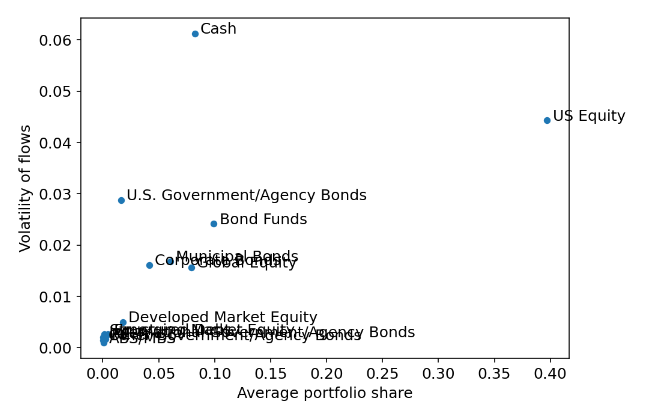
\includegraphics[width=0.7\linewidth]{screenshot001}
		\end{center}		
		Figure 12 (reproduced above) suffers from an issue of illegibility. Some labels are illegible due to overlapping text and markers. Furthermore, the marker for \textit{US Equity} overlaps the frame of the figure. I recommend that the authors ensure that all labels are readable. Consider adjusting the font size or using a different layout to prevent overlap.
		
	
		\begin{center}
			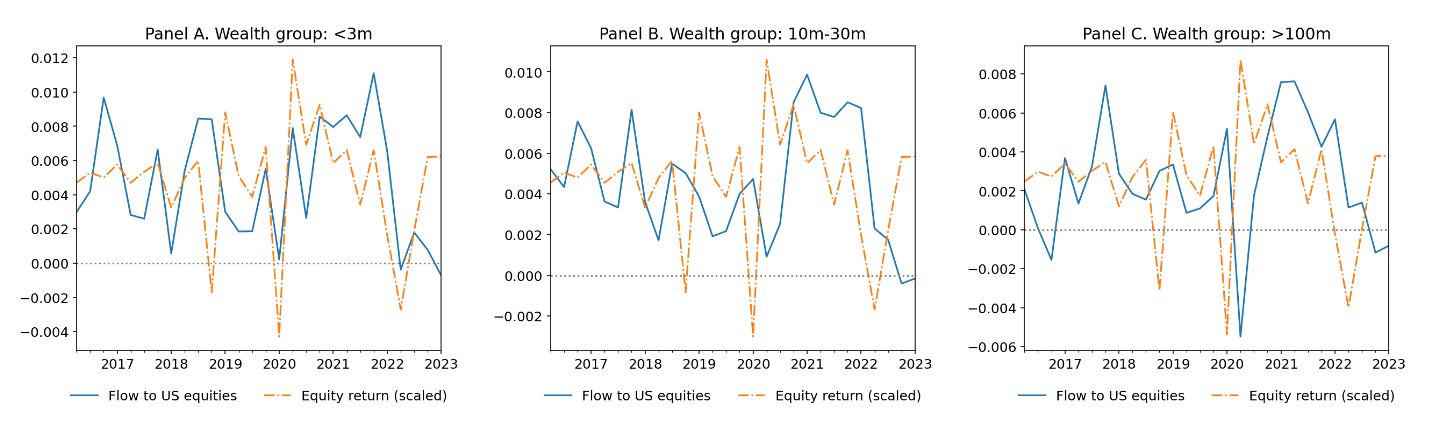
\includegraphics[width=\linewidth]{screenshot002}
		\end{center}
		Figures 15 (reproduced above) and 16 are both similarly represented in the paper. Three graphs presented side by side. However, at a glance these visualizations are hard to read. The thin texts and lines make it difficult to distinguish between different elements in the graphs, impacting the overall clarity and readability of the figures. Enhancing the contrast between the lines and the background, as well as using bolder fonts for the text labels, could significantly improve the legibility of these visualizations. Additionally, stacking the graphs vertically rather than horizontally would allow each graph to be bigger and more legible.
	
		


\pagebreak
\printbibliography

\end{spacing}
\end{document}
